\begin{section}{Problem 5}
    \begin{problem}{5}
        The following picture appears in \textsc{Matlab's} repository of images, and can be retrieved by entering 
        \begin{verbatim}
    load mandrill; 
    colormap('gray'); 
    image(X);
        \end{verbatim}
        \begin{center}
            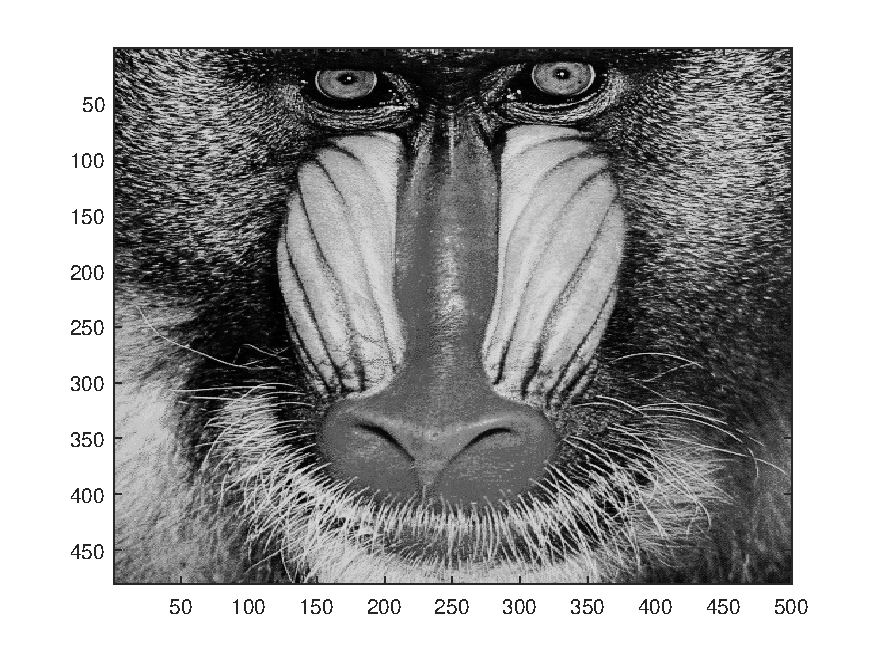
\includegraphics[scale=0.7]{mandrill2.pdf}
        \end{center}
        
        \begin{enumerate}[(a)]
            \item Print out the images generated by the truncated SVD. Start with $r=2$ and go up by powers of $2$, to $r=2^6=64$ (six plots in total). For a compact presentation of your figures, you may use the command {\tt subplot(3,2)}. (Check out {\tt help subplot}.)        
            \item Comment briefly on the quality of the images as a function of $r$. For what value of $r$ would you say that the quality of the image is acceptable, in that we can be rather confident of what we are seeing? (We are not looking for a specific ``correct answer'' here - just make your subjective observation.)
            \item For the value of $r$ you stated in part (b), how much storage is required? Compare it to the storage required for the original image.
        \end{enumerate}
    \end{problem}

    \newpage

    \begin{solution}{a}
        \begin{mdframed}
            \footnotesize
            \textbf{File: {\tt DevamSisodraker\_5a.m}}
            \inputminted{matlab}{DevamSisodraker_5a.m}
            \normalfont
        \end{mdframed}

        \continued

        \begin{mdframed}
            \footnotesize
            \textbf{File: {\tt DevamSisodraker\_5a\_out.txt}}
            \inputminted{matlab}{DevamSisodraker_5a_out.txt}
            \normalfont
        \end{mdframed}

        \continued

        \begin{mdframed}
            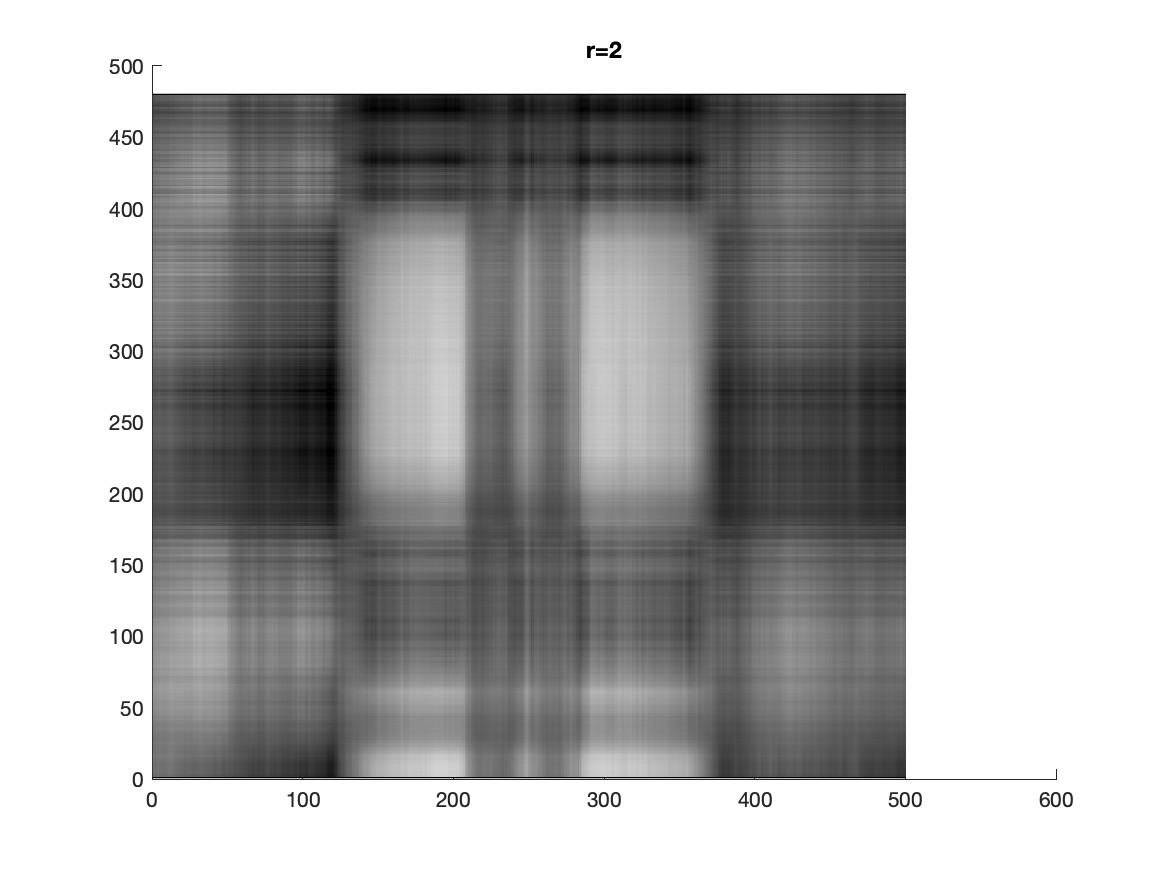
\includegraphics[scale=0.33]{DevamSisodraker_5a_2.jpg}
        \end{mdframed}

        \continued

        \begin{mdframed}
            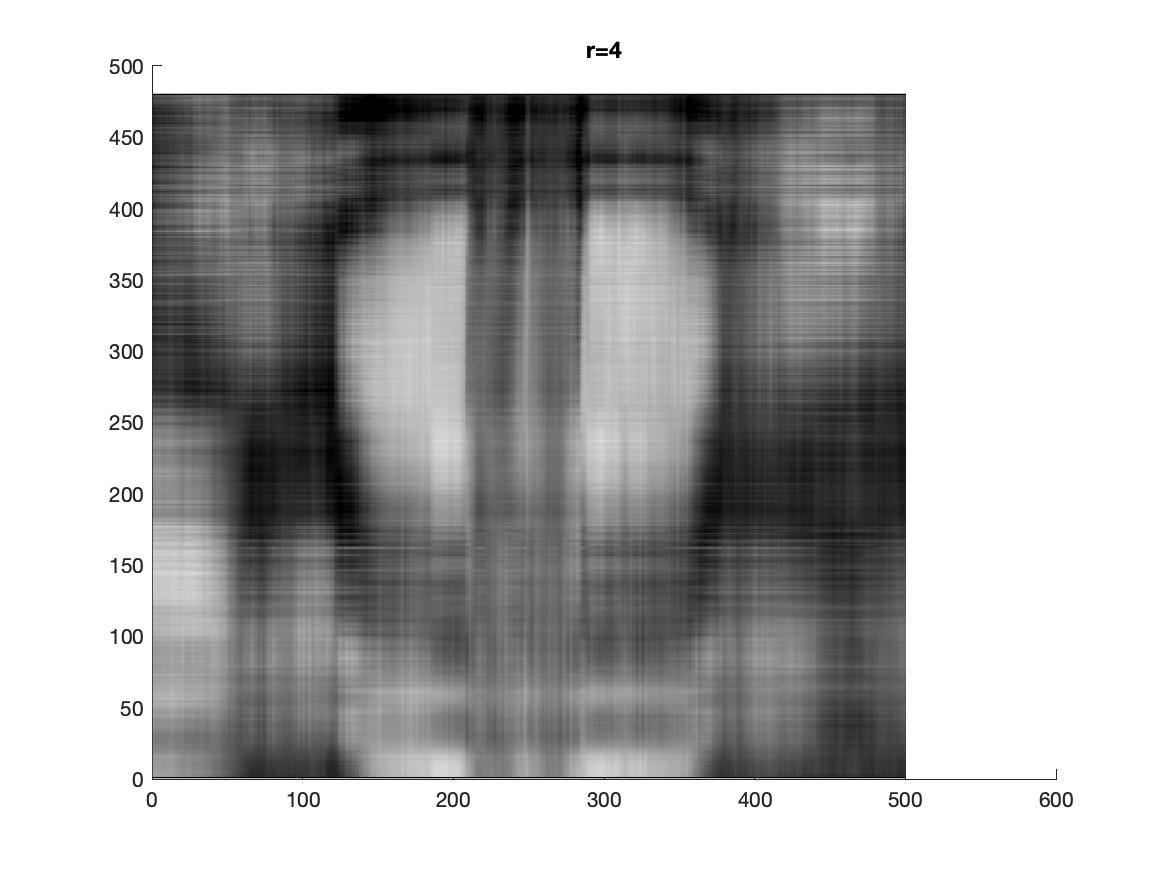
\includegraphics[scale=0.33]{DevamSisodraker_5a_4.jpg}
        \end{mdframed}

        \continued

        \begin{mdframed}
            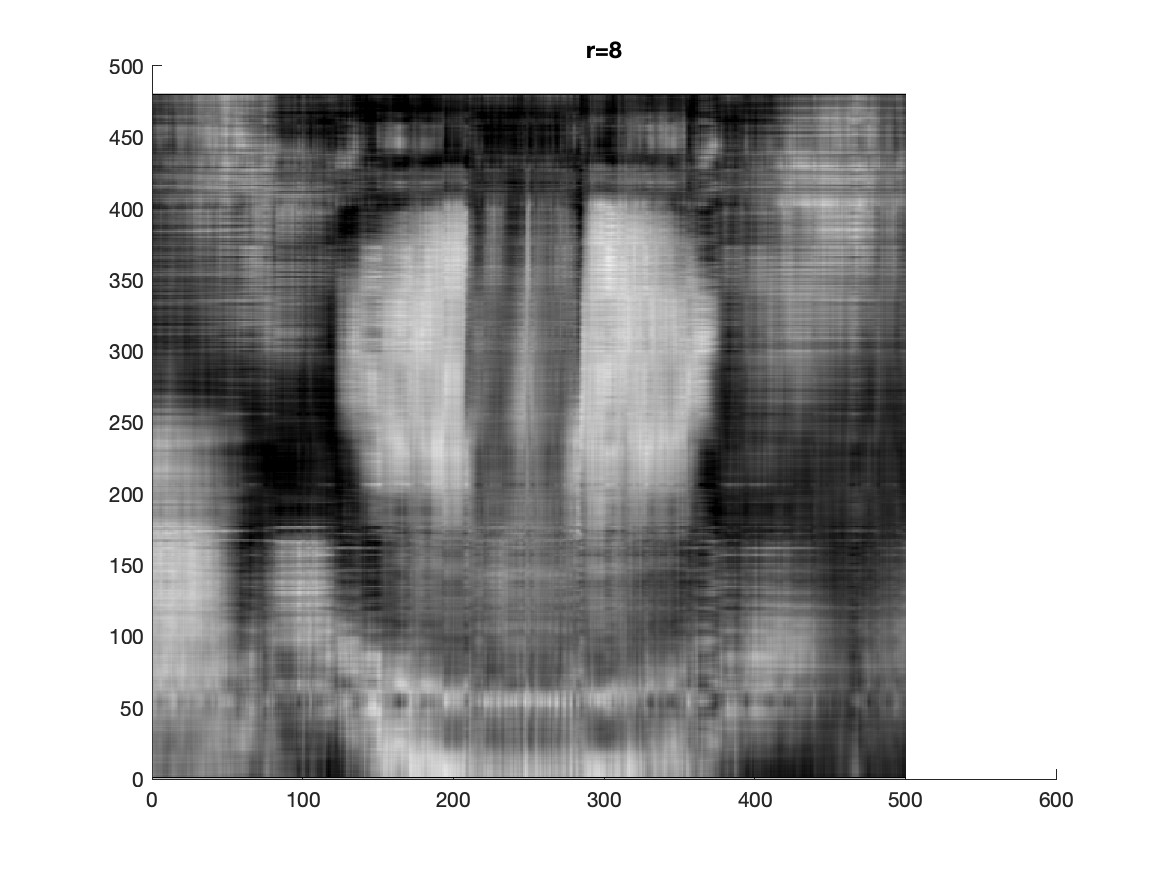
\includegraphics[scale=0.33]{DevamSisodraker_5a_8.jpg}
        \end{mdframed}

        \continued

        \begin{mdframed}
            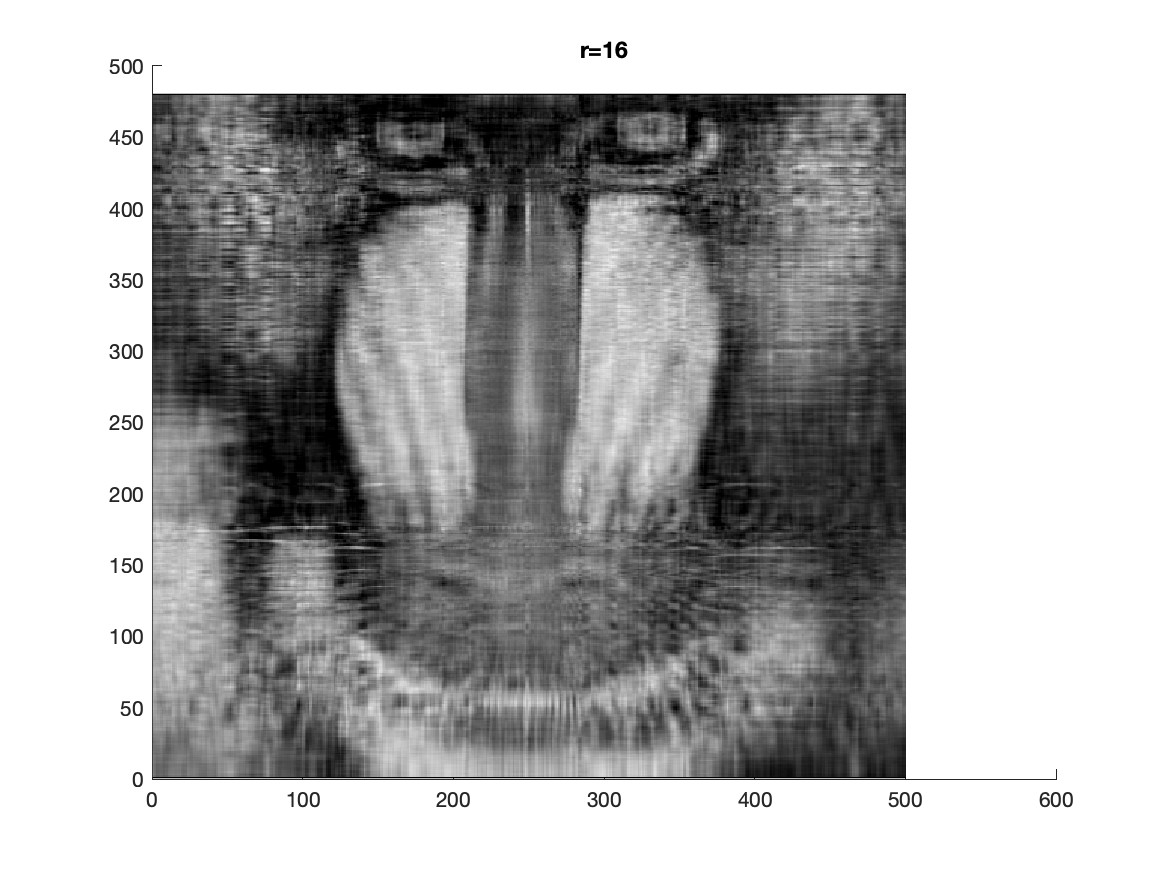
\includegraphics[scale=0.33]{DevamSisodraker_5a_16.jpg}
        \end{mdframed}

        \continued

        \begin{mdframed}
            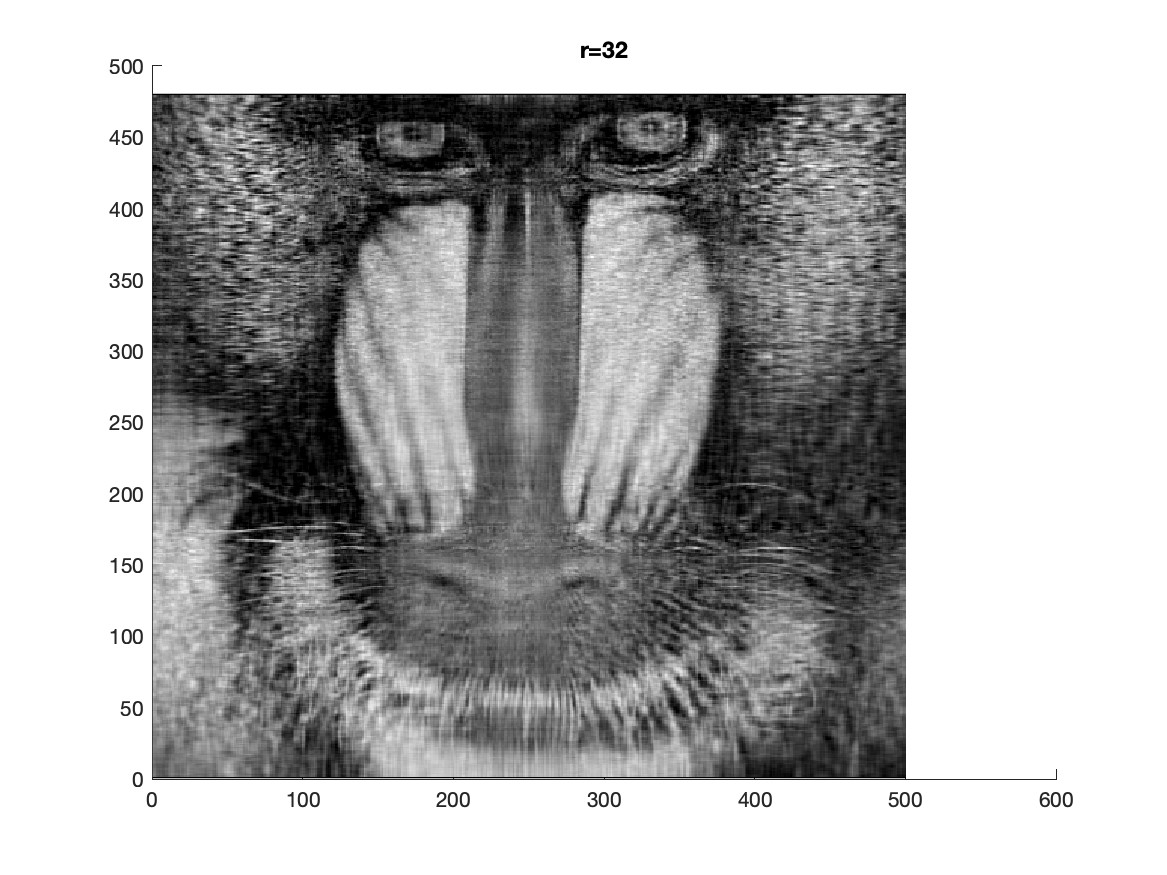
\includegraphics[scale=0.33]{DevamSisodraker_5a_32.jpg}
        \end{mdframed}

        \continued

        \begin{mdframed}
            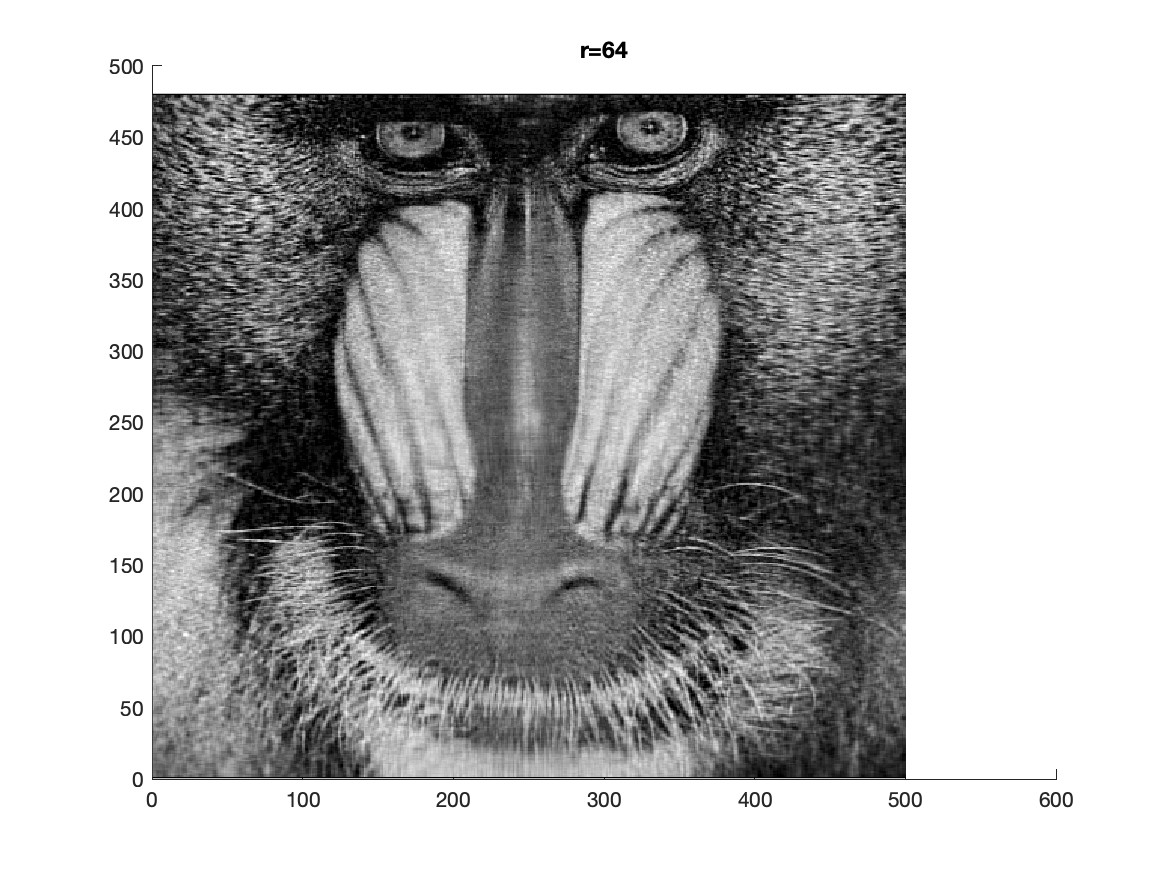
\includegraphics[scale=0.33]{DevamSisodraker_5a_64.jpg}
        \end{mdframed}
    \end{solution}

    \newpage
    
    \begin{solution}{b}
        While we can start to discern the original image when $r = 16$, it is still possible to notice various obvious abnormalities in the image produced (including various lines and inconsistencies around the bottom of the image). Therefore I choose $r = 32$ to be (in my subjective opinion) to be "acceptable" since it clearly shows us a very close depiction of the original image.
    \end{solution}

    \begin{solution}{c}
        Since the amount of significant singular values of a matrix effectively determines what its "rank" is, then we only require space to store the $32$ column vectors of $U$ and $V$ ($32$ vectors each) that are associated with the $32$ singular values (as dictated by the value of $r$). Thus it costs $32 \cdot (480 + 500 + 1) = 31392$ "units" of storage versus the original image which costs $480^2 + 500^2 + 480 = 480880$ "units" of storage. When $r = 32$ we use around $\frac{480880}{31392} \approx 15$ times less storage.
    \end{solution}
\end{section}